\documentclass[twocolumn]{article}
\usepackage{cite}
\usepackage{graphicx} % Required for inserting images
\usepackage{color}
\usepackage{lineno}
\usepackage[affil-it]{authblk}
\usepackage{amsmath}
\usepackage{amssymb}
\usepackage{comment}
\usepackage{float}
\usepackage{xparse} % for custom commands
\usepackage{abstract} % needed for custom author footnotes/thanks
\usepackage{subcaption}
\usepackage{hyperref}
\hypersetup{%
     colorlinks=true,
     linkcolor=blue,
     filecolor=blue,
     citecolor = red,
     urlcolor=cyan,
     }
\usepackage[ruled,linesnumbered]{algorithm2e}
\usepackage{xargs}
\usepackage{xcolor}
%\usepackage{sistyle}
\usepackage{siunitx}
%\SIthousandsep{,}
\usepackage{tikz}
\usetikzlibrary{calc}
\usetikzlibrary{shapes.geometric}
\usepackage[textsize=tiny]{todonotes}
\setlength{\marginparwidth}{2cm} % required for todonotes in twocolumn
\newcommandx{\PCunsure}[2][1=]{\todo[linecolor=red,backgroundcolor=red!25,bordercolor=red,#1]{#2~-PC}}
\newcommandx{\PCchange}[2][1=]{\todo[linecolor=blue,backgroundcolor=blue!25,bordercolor=blue,#1]{#2~-PC}}
\newcommandx{\PCinfo}[2][1=]{\todo[linecolor=green,backgroundcolor=green!25,bordercolor=green,#1]{#2~-PC}}
\newcommandx{\PCimprovement}[2][1=]{\todo[linecolor=magenta,backgroundcolor=magenta!25,bordercolor=magenta,#1]{#2~-PC}}
\newcommandx{\DJunsure}[2][1=]{\todo[linecolor=red,backgroundcolor=red!25,bordercolor=red,#1]{#2~-DJ}}
\newcommandx{\DJchange}[2][1=]{\todo[linecolor=blue,backgroundcolor=blue!25,bordercolor=blue,#1]{#2~-DJ}}
\newcommandx{\DJinfo}[2][1=]{\todo[linecolor=green,backgroundcolor=green!25,bordercolor=green,#1]{#2~-DJ}}
\newcommandx{\DJimprovement}[2][1=]{\todo[linecolor=magenta,backgroundcolor=magenta!25,bordercolor=magenta,#1]{#2~-DJ}}
\newcommandx{\MHJimprovement}[2][1=]{\todo[linecolor=magenta,backgroundcolor=magenta!25,bordercolor=magenta,#1]{#2~-MHJ}}
\newcommand{\citationneeded}{\textsuperscript{\color{red} [citation needed]}}

\def\IsInteger#1{%
  TT\fi
  \begingroup \lccode`\-=`\0 \lccode`+=`\0
    \lccode`\1=`\0 \lccode`\2=`\0 \lccode`\3=`\0
    \lccode`\4=`\0 \lccode`\5=`\0 \lccode`\6=`\0
    \lccode`\7=`\0 \lccode`\8=`\0 \lccode`\9=`\0
  \lowercase{\endgroup
    \expandafter\ifx\expandafter\delimiter
    \romannumeral0\string#1}\delimiter
}
\newcommand{\ord}[1]{%
    \if\IsInteger{#1}%
        \ifthenelse{1=#1}
        {%
            $1^{\mathrm{st}}$%
        }%
        {%
            \ifthenelse{2=#1}
            {%
                $2^{\mathrm{nd}}$%
            }%
            {%
                \ifthenelse{3=#1}
                {%
                    $3^{\mathrm{rd}}$%
                }%
                {%
                    $#1^{\mathrm{th}}$%
                }%
            }%
        }%
    \else%
        {%
            $#1^{\mathrm{th}}$%
        }%
    \fi%
}
\NewDocumentCommand{\expectation}{m o}{%
\IfValueTF{#2}{%
    \ensuremath{\left\langle #1 \middle| #2 \middle| #1\right\rangle}%
}
{%
    \ensuremath{\left\langle #1 \right\rangle}%
}
}
\NewDocumentCommand{\nxn}{o}{%
\IfValueTF{#1}{%
    \ensuremath{#1 \times #1}
}
{%
    \ensuremath{n \times n}
}
}
%\newcommand{\nxn}[1]{\ensuremath{#1 \times #1}}
\newcommand{\bra}[1]{\ensuremath{\left\langle #1 \right|}}
\newcommand{\ket}[1]{\ensuremath{\left| #1 \right\rangle}}
\newcommand{\braket}[2]{\ensuremath{\left\langle #1 \middle| #2 \right\rangle}}
\newcommand{\ketbra}[2]{\ensuremath{\left| #1 \right\rangle\left\langle #2 \right|}}
\newcommand{\Mvecc}{\ensuremath{M\left(\vec{c}\,\right)}}
\newcommand{\Nmax}{\ensuremath{N_{\mathrm{max}}}}
\newcommand{\bigO}[1]{\ensuremath{\mathcal{O}\left(#1\right)}}
\newcommand{\tenS}{\ensuremath{\mathcal{S}}}
\newcommand{\tenP}{\ensuremath{\mathcal{P}}}
\newcommand{\tenQ}{\ensuremath{\mathcal{Q}}}
\newcommand{\tenN}{\ensuremath{\mathcal{N}}}
\newcommand{\expm}[1]{\ensuremath{\mathrm{exp}\left\{#1\right\}}}


\newcommand{\MSU}{Department of Physics and Astronomy, Michigan State University, East Lansing, Michigan 48824}
\newcommand{\CMSE}{Department of Computational Mathematics, Science and Engineering, Michigan State University, East Lansing, Michigan 48824}
\newcommand{\FRIB}{Facility for Rare Isotope Beams, Michigan State University, East Lansing, Michigan 48824}
\newcommand{\Oslo}{Department of Physics and Center for Computing in Science Education, University of Oslo, N-0316 Oslo, Norway}
\newcommand{\Cornell}{Department of Electrical and Computer Engineering, Cornell Tech, New York, NY 10044}

\begin{document}

%\linenumbers
\title{Parametric Matrix Models}

\author[1,2]{Patrick Cook\footnote{Contributed equally}\thanks{\texttt{cookpat4@msu.edu}; Corresponding author}}

% the following disaster seems to be the only good way to get the same * footnote with two corresponding authors
\newcommand\CoAuthorMark{\addtocounter{footnote}{-1}\footnotemark[\arabic{footnote}]\addtocounter{footnote}{1}}

\author[1,2]{Danny Jammooa\protect\CoAuthorMark\thanks{\texttt{jammooa@frib.msu.edu}; Corresponding author}}

\author[2,1,3]{Morten~Hjorth-Jensen}

\author[4]{Daniel~D.~Lee}

\author[2,1]{Dean~Lee}

\affil[1]{\MSU}
\affil[2]{\FRIB}
%\affil[3]{\CMSE}
\affil[3]{\Oslo}
\affil[4]{\Cornell}

\date{\today} % it's always \today, today

\twocolumn[
  \begin{@twocolumnfalse}
    \maketitle
    \begin{abstract}
       We present a general class of machine learning algorithms called parametric matrix models. Parametric matrix models are based on matrix equations, and the design is motivated by the efficiency of reduced basis methods for approximating solutions of parametric equations.  The dependent variables can be defined implicitly or explicitly, and the equations may use algebraic, differential, or integral relations.   Parametric matrix models can be trained with empirical data only, and no high-fidelity model calculations are needed.  While originally designed for scientific computing, parametric matrix models are universal function approximators that can be applied to general machine learning problems.  After introducing the underlying theory, we apply parametric matrix models to a series of different challenges that show their performance for a wide range of problems.  For all the challenges tested here, parametric matrix models produce accurate results within a computational framework that allows for parameter extrapolation and interpretability.
    \end{abstract}
  \end{@twocolumnfalse}]

\saythanks

%########################################
\section{Introduction}

%\PCunsure{I removed Danny and my CMSE affiliation: does a dual PhD really mean we're in that department? - Dean: done}
%\PCimprovement{ABSTRACT: Add some sort of mention that PMMs require significatly fewer hyperparameters in practice. - Dean: done} 
Any machine learning algorithm can be expressed as a set of constraint equations, $\vec{F}(\vec{c},\vec{m},\vec{y})=0$, connecting input parameters $\vec{c}$, model parameters $\vec{m}$ to be learned, and dependent variables $\vec{y}$ comprising intermediate and final outputs.  For example, the constraint equations may enforce the minimization of some specific loss function.  For essentially all machine learning approaches, the constraint equations involve explicit relations defining each dependent variable.  However, one can also consider constraint equations where the dependent variables are defined implicitly \cite{chen2018neural,bai2019deep,zhang2019equilibrated,kag2019rnns,gu2020fenchel,el2021implicit}. Here we introduce a general class of machine learning algorithms called parametric matrix models (PMMs), where the constraint equations to be solved are matrix equations. The dependent variables can be defined implicitly or explicitly, and the equations may use algebraic, differential, or integral relations.  One very simple example is  $M(\vec{c}) = M_0 + \sum_i c_i M_i$, where $M_0$ and each $M_i$ are Hermitian matrices, and the final outputs are eigenvalues of $M(\vec{c})$.  The PMM can be designed to incorporate as much mathematical and scientific insight as possible or used more broadly as a universal function approximator that can be efficiently optimized.  In practice, PMMs typically need fewer hyperparameters to tune as compared with other machine learning approaches, therefore requiring less fine-tuning and model crafting.  This efficiency of description does not imply a loss of generality or flexibility. It is instead the result of a natural design that prioritizes functions with the simplest possible analytic properties when continued into the complex plane.  
%\PCunsure{I would say that PMMs are a hybrid data- and theory- driven approach. Consider regularization; instead of relying purely on the behavior of the data or of the output, we are able to use the underlying mathematical properties.  - Dean: Wording changed to reflect this.} 
While PMMs use data-driven methods, they also borrow the mathematical structure of theory-based model-driven approaches such as reduced basis methods \cite{quarteroni2015reduced,hesthaven2015certified} without the need for model data.  
Such an approach is already used in dynamic mode decomposition \cite{SCHMID_2010,tu2013dynamic,proctor2016dynamic,kutz2016dynamic} for dynamical systems with coupled spatial and temporal modes. Matrix-based approaches have also been widely used in machine learning for dimensionality reduction 
\cite{lee2000algorithms,wang2012nonnegative,saul2022geometrical}. This work introduces the general strategy of PMMs and shows the utility of PMMs for a broader class of problems. 

To illustrate this, we consider the recently introduced eigenvector continuation (EC) method\cite{DFrame,Demol:2019yjt,Konig:2019adq,Ekstrom:2019lss,Furnstahl:2020abp,Sarkar:2020mad,Duguet:2023wuh,Hicks:2022ovs}. Eigenvector continuation is a reduced basis method that finds the eigenvectors and eigenvalues for a parameterized family of Hermitian matrices $H(\vec{c})$ whose elements are analytic functions of $\vec{c}$.  The EC calculation starts by picking some set of eigenvectors $\ket{v_j(\vec{c}_i)}$ at selected values $\vec{c}\in\left\{\vec{c}_i\right\}$.  It then projects all vectors to the subspace spanned by these eigenvector snapshots. The task then reduces to finding the eigenvalues and eigenvectors of a much smaller Hermitian matrix $M(\vec{c})$, whose elements are also analytic functions of $\vec{c}$.  The eigenvalues are roots of the characteristic polynomial, $\det [M(\vec{c})-\lambda \mathbb{I}]$. If we approximate the dependence on $\vec{c}$ over some $d$-dimensional compact domain using polynomials, then each $\lambda$ corresponds to the roots of a polynomial in $\lambda$ with coefficients that are polynomials with respect to $\vec{c}$.

The resulting algebraic variety defining $\lambda$ is endowed with some very useful properties.  For all real values of  $\vec{c}$, $\lambda$ will be analytic and bounded by the norm of $M(\vec{c})$, which is a polynomial in $\vec{c}$.  Using only general arguments of analyticity, in Ref.~\cite{Duguet:2023wuh} it is shown that with $N_b$ basis vectors, the error of the EC approximation diminishes as a decaying exponential function of $N_b^{1/d}$ in the limit of large $N_b$. For the case of eigenvalue problems, PMMs capture the essential features of the EC calculations by proposing some unknown Hermitian matrix $M(\vec{c})$ and learning the polynomials in $\vec{c}$ that comprise its matrix elements.  

The PMMs can achieve the same rapid convergence with matrix dimension as EC for eigenvalue problems.  A constructive proof is to tune the matrix parameters to the same matrix $M(\vec{c})$ corresponding to an EC calculation.  However, this is not how PMMs will typically be used.  A key computational advantage of PMMs is that they can be trained with empirical data only.  No high-fidelity model calculations are needed.  Despite starting with less information, there are many examples where PMMs still achieve superior performance when compared with EC. 

For example, we consider first a simple system composed of $N$ non-interacting spin-$1/2$ particles with the one-parameter Hamiltonian 
\begin{equation}\label{eq:nonintH}
H(c) = \frac{1}{2N}\sum_i^N \left(\sigma^z_i + c\sigma^x_i \right).
\end{equation}
Here, $\sigma^z_i$ and $\sigma^x_i$ are the $z$ and $x$ Pauli matrices for spin $i$, respectively. We see in Fig.~\ref{fig:EC_PMM}, that the EC method has difficulties in reproducing the ground state energy $E_0$ for large $N$ using five training points, or snapshots, which here are the eigenpairs obtained  from the  solution  of the full $N$-spin problem.  The PMM representation does not have this problem and is able to exactly reproduce $E_0$ for all $N$ using a learned $\nxn[2]$ matrix model only of the  form $M(c) = \left(\sigma^z + c\sigma^x \right)/2$.  While this particular example is a rather trivial non-interacting system, it illustrates the general principle that PMMs have more freedom than reduced basis methods.  They do not need to correspond to a projection onto a fixed subspace, and this allows for efficient solutions to describe a wider class of problems.

The eigenvalue problem is only one example among many from a very broad class of problems that PMMs can address.  For scientific computing applications, the general strategy is to incorporate as much of the underlying science and applied mathematics into the structure of the PMM.  However, PMMs can also be used for general problems outside the domain of scientific computing.  The PMMs we have just discussed can output any polynomial function of the input parameters, and therefore the universal function approximation condition is guaranteed by the Weierstrass approximation theorem \cite{BrinkhuisTikhomirov2006}.
\begin{figure}[ht]
    \centering
    \includegraphics[width=\columnwidth]{./Figures/EC_PMM.pdf}
    \caption{\label{fig:EC_PMM}Results for the ground state energy of the Hamiltonian given by Eq.~\eqref{eq:nonintH} as a function of the interaction strength parameter $c$. Extrapolated results from the $5$ training points (diamond symbols) located where $c<0$ are shown for EC (dotted red) and a $\nxn[2]$ PMM (dashed blue). The exact ground state energy is shown in solid black.
 }
\end{figure}


We outline here the rest of this work. In the next section, in order to benchmark the performance and the versatility of PMMs, we consider three very different examples of interest to a broader audience.  For each case, we compare the PMMs against other state-of-the-art methods.  
Our conclusions and perspectives for future studies are presented in the subsequent section. We also include several additional examples in the supplementary material. 

\section{Performance and Versatility of Parametric Matrix Models}
In this section we showcase the performance and versatility of PMMs by applying the method to three distinct problems. The examples we consider are the energy levels of the quantum anharmonic oscillator (Sec.~\ref{sec:AHO}), the extrapolation of the so-called Trotter approximation errors in quantum computing (Sec.~\ref{sec:trotter}), and finally the unsupervised image clustering of handwritten digits (Sec.~\ref{sec:unsupervised}).

\subsection{Quantum Anharmonic Oscillator\label{sec:AHO}}
The quantum anharmonic oscillator describes the quantum mechanics of a particle confined by an external potential of the form $V(x)= \frac{1}{2}k x^2 + \lambda x^4$.  The corresponding scaled Hamiltonian can be written as
\begin{equation}
    \label{eq:anharm}
    H(g) = a^\dagger a + g\left(a^\dagger + a\right)^4,
\end{equation}
where $a^\dagger$ and $a$ are creation and annihilation operators  
satisfying the relation $a a^\dagger- a^\dagger a = 1$.  We have absorbed multiplicative and additive constants into the definition of $H$, and the relative anharmonicity is represented by the dimensionless parameter $g$.  This model has attracted much interest and has been the subject of many theoretical and computational studies throughout the years~\cite{mcweeny1948quantum,banerjee1978anharmonic,feranchuk1995operator,bender1996multiple,jafarpour2001calculation,franzke2022excited}.

The quantum anharmonic oscillator has a complicated analytical structure with an infinite number of branch points in the complex plane that accumulate at $g=0$~\cite{PhysRev.184.1231}. While the Hamiltonian is unbounded below for $g<0$, applying a finite truncation of the basis states allows the Hamiltonian to be defined for all $g$.  We perform this truncation using harmonic oscillator eigenstates corresponding to $H(g=0)=H(0)$ and make the restriction of maximum energy excitation $N_{\rm max}$.  For the example considered here, we take $N_{\rm max}=100$.  For $g<0$, there are large negative potential energies of equal depth for large positive $x$ and large negative $x$. As a result, there is an approximate degeneracy of positive and negative parity states for $g<0$.  The energy gap between the lowest two energy states, $E_1 - E_0$,
%, and the number operator $\hat{n} = a^\dagger a$ are 
provides a useful probe of this degeneracy for $g<0$ and the change in character as we cross $g=0$.  

We compare here the performance of a multilayer perceptron (MLP) neural network \cite{goodfellow2016} and cubic spline interpolation \cite{Stoer1993} with our PMM approach in learning the lowest two energy levels $E_0$ and $E_1$ as a function of $g$~\cite{Stoer1993}.  For each case, we provide training data for $E_0$ and $E_1$ at ten evenly-spaced values of $g$, spanning the range $g\in [-0.01,0.01]$ and for validation data approximately $100$ evenly-spaced points throughout the same domain. The validation set was withheld during training and only used to stop training before overfitting. The MLP we compared to used the rectified linear unit \cite{goodfellow2016} as the activation function and had two hidden layers of $25$ neurons each. We trained $\num{100}$ of these MLPs and show the average results. For the cubic spline analysis, we applied the standard approach with zero curvature at the end points.  For the PMM, we use a $\nxn[5]$ matrix model and use the matrix structure we would get from applying EC to the quantum anharmonic oscillator, $M(g)=M_0 + gM_1$, where $M_0$ and $M_1$ are Hermitian matrices.  Using the unitary transformation to diagonalize $M_0$, we can simplify further to the form $M(g)=D + gM'_1$, where $D$ is a real diagonal matrix.  All of the nonzero entries of $D$ and $M'_1$ are learned by fitting the two lowest eigenvalues of $M(g)$ to the training data.

Figure~\ref{fig:AHOPMM} shows the results for the three different approaches in comparison with the exact results.  We see that the PMM performs significantly better than both the MLP and cubic spline.  The superior performance is not specific to the example considered here.  The PMM has the advantage that it learns the underlying physics of branch point singularities in the complex plane of $g$ near the real axis \cite{Kato:1966:PTL}. We further explore this property of PMMs---as well as their ability to learn observables associated with the system---in the Supplemental Material.
\begin{figure*}[ht]
    \centering
    \includegraphics[width=0.7\linewidth]{./Figures/AHO.pdf}
    \caption{\label{fig:AHOPMM}The two lowest two energies of the quantum anharmonic oscillator as a function of $g$ (top) and the absolute error in the three methods used to interpolate the training data (bottom). The main figure focuses on the region of interest where the degeneracy between the first two levels is first broken. The inset shows the full domain of $0.01\leq g \leq 0.01$ with the focused region highlighted. These results show that not only does the PMM outperform MLP and cubic splines, but guarantees the preservation of important basic properties like level ordering where the other methods do not.}
\end{figure*}


%########################################
\subsection{Zero Trotter Step Extrapolation\label{sec:trotter}}
One of the primary challenges in quantum computing is determining observables of interest while using circuits with as few qubits and quantum gates as possible.  This minimal resource strategy is necessary due to the limitations of noise and decoherence~\cite{leymann2020bitter}.

There are several efficient algorithms that determine energy levels on a quantum computer using the complex phases produced during the time evolution of quantum states \cite{Kitaev:1995qy,Abrams:1997gk,dorner2009optimal,Svore:2013fci,Choi:2020pdg,RuizGuzman:2021qyj,Qian:2021wya,Bee-Lindgren:2022nqb,Cohen:2023rhd}.  
The time evolution operator for time duration $t$ corresponds to the exponential of the Hamiltonian, $\expm{-iHt}$. This is implemented as a product of evolution operators for small time steps $dt$, $\expm{-iHdt}\cdots \expm{-iHdt}$.  Each term $U(dt) = \expm{-iHdt}$ can be approximated as a product of exponentials of the individual terms comprising $H$.  This approximation becomes exact in the limit $dt \rightarrow 0$ and is known as a Trotter product \cite{trotter1959product}, and the generalization to products with higher-order errors in $dt$ are called Trotter-Suzuki formulae \cite{Suzuki:1976,Suzuki:1993,childs2021theory}.

The desired energies $E_k$ are determined by setting $\expm{-iE_kdt}$ equal to the eigenvalues of $U(dt)$ and extrapolating to the limit $dt \rightarrow 0$.  Data from small $dt$ are often not possible due to the large number of quantum gates required.  Several polynomial interpolation and extrapolation methods have therefore been developed \cite{Endo:2019,vazquez2022enhancing,Rendon:2022csn}. In the following, we use PMMs to determine $E_k$ and compare with polynomial interpolation methods.

We consider a one-dimensional quantum spin chain with nearest and next-to-nearest neighbor interactions. The Hamiltonian of this Heisenberg system is ${H=H_B + H_{J_1}^0 + H_{J_1}^1 + H_{J_2}^0 + H_{J_2}^1}$, where
\begin{equation}
\label{eq:NN}
\begin{aligned}
    H_B&=B\sum_i^N r_i\sigma_i^z\\
    H_{J_1}^{0|1}&=J_1\sum_{i\,\rm even|odd}^N(\sigma_i^x\sigma_{i+1}^x + \sigma_i^y\sigma_{i+1}^y+ \sigma_i^z\sigma_{i+1}^z) \\
    H_{J_2}^{0|1}&=J_2\sum_{i\,\rm even|odd}^N(\sigma_i^x\sigma_{i+2}^x + \sigma_i^y\sigma_{i+2}^y+ \sigma_i^z\sigma_{i+2}^z),
\end{aligned}
\end{equation}
where $r_i$ are random real numbers ranging from $[0,1)$. For $U(dt)$, we use the Trotter product
\begin{equation}
\begin{aligned}
    U(dt) &= \expm{-iH_Bdt}\expm{-iH_{J_1}^0dt}\\&\times\expm{-iH_{J_1}^1dt}\expm{-iH_{J_2}^0dt}\\&\times\expm{-iH_{J_2}^1dt}.
\end{aligned}
\end{equation}
We use a PMM with the same underlying structure,
\begin{equation}
\begin{aligned}
    U_M(dt) &= \expm{-iM_1dt} \expm{-iM_2dt}\\&\times\expm{-iM_3dt}\expm{-iM_4dt}\\&\times\expm{-iM_5dt},
\end{aligned}
\end{equation}
where each of the matrices, $M_i$, are $\nxn[10]$ Hermitian matrices. We use the values $B=J_1=1$, and $J_2=0.5$, and choose 10 values of $dt$ spanning the range $[-0.18,-0.15]\cup[0.15,0.18]$.  We train the PMM using the ground state, first excited state, and second excited state for $N=8$ qubits with periodic boundary conditions.
\begin{figure}
    \centering
\includegraphics[width=\columnwidth]{./Figures/Trotter_NN.pdf}
    \caption{\label{fig:trotter2}Results for selected energy levels in the one-dimensional Heisenberg spin chain with nearest-neighbor and next-nearest-neighbor interactions (top) as well as the relative error for the extrapolated values at $dt=0$ (bottom). We show the $\nxn[10]$ PMM results (dashed lines, square diamonds), polynomial interpolation results (dotted lines, squares), exact diagonalization calculation of Trotter ground-truth (solid lines), and Trotter training data (thin diamonds). The vertical grey line highlights $dt=0$.}
\end{figure}

Using the same training data, we compare the PMM results with polynomial interpolation.  Since we do not have data at smaller values of $dt$, the polynomial fitting is less reliable than the Chebyshev polynomial interpolation used in Ref.~\cite{rendon2023improved}.  The results are shown in Fig.~\ref{fig:trotter2}. Polynomial interpolation was not able to handle the sharp avoided level crossings involving the first and second excited states. In contrast, the PMM reproduces the avoided level crossings properly---which are not present in the training data---and also predicts the first and second excited states at $dt = 0$ with much higher accuracy.



%########################################

\subsection{Unsupervised Image Clustering}\label{sec:unsupervised}
To demonstrate the usefulness of PMMs beyond scientific computing---in areas that are dominated by neural networks---we apply a PMM to the problem of unsupervised image clustering on the MNIST dataset. This dataset consists of \num{60000} (\num{10000}) labeled training (test) $\nxn[28]$ monochrome images of handwritten digits from $0$ to $9$. The goal of an unsupervised learning algorithm on this dataset is to---without the use of any data labels---project this data from the original $\nxn[28] = 784$ dimensional space to a significantly lower dimensional space, often to just $2$ dimensions. This projection should cluster similar images together in the low dimensional space, effectively identifying the $10$ different digits without knowing what image is what digit, or even that there are $10$ digits.

We apply an $\nxn[8]$ PMM of the form ${M(\vec{c}) = D + \sum_{i=1}^{784} c_iM_i}$, where $D$ is a real diagonal matrix and $M_i$ are complex hermitian matrices whose individual matrix elements are drawn from a tensor network in order to drastically reduce the number of training parameters. The details of this tensor network PMM are described in the Supplementary Material Sec.~\ref{sec:TN}. Results both with and without this tensor network formulation were qualitatively and quantitatively indistinguishable. We trained the PMM using only \num{10000} images from the training set. For each image $\vec{c}$, the projected output was taken to be the two most-interior eigenvalues of the PMM $M(\vec{c})$. Training the PMM is done in a manner similar to t-distributed Stochastic Neighbor Embedding (t-SNE) by minimizing the Kullback-Leibler divergence between the original data and the projected data~\cite{vanderMaaten08}. Figure~\ref{fig:mnist} shows the results of the learned embedding by a PMM applied to the training data as well as \num{10000} images from the MNIST test set which were unseen during training. Table~\ref{tbl:MNIST} shows the 1-nearest-neighbor generalization error of our embedding compared to Principal Component Analysis (PCA), a supervised technique known as Neighborhood Components Analysis (NCA), an autoencoder, and parametric t-SNE~\cite{vanderMaaten09, Goldberger04}. The 1-nearest-neighbor generalization error measures the percentage of nearest neighbor pairs in the low-dimensional embedding which were not part of the same class. An important note is that we did not preprocess the original dataset in any way as is usually done when using t-SNE-like methods to reduce the dimensionality of the training data~\cite{vanderMaaten08, vanderMaaten14}. Our results demonstrate that a PMM is able to produce a high-quality parametric embedding, which basic t-SNE methods alone cannot do without preprocessing, pretraining, and finetuning~\cite{vanderMaaten09}. Moreover, these results demonstrate the utility of PMMs beyond scientific computing.

\begin{table*}[ht]
\centering
    \begin{tabular}{|l p{2cm} S[table-format=2.2] S[table-format=2.2] r|}
\hline
        \textbf{Method} & \textbf{Training\newline Examples} & \textbf{Train Error} & \textbf{Test Error} & \textbf{Source}\\
\hline
\hline
        PCA & \num{60000} & $\textrm{---}$ & 78.16\% & \cite{vanderMaaten09}\\
        NCA & \num{60000} & $\textrm{---}$ & 56.84\% & \cite{vanderMaaten09}\\
        Autoencoder & \num{60000} & $\textrm{---}$ & 66.84\% & \cite{vanderMaaten09}\\
        Par.\ t-SNE & \num{60000} & $\textrm{---}$ & 9.90\% & \cite{vanderMaaten09}\\
\hline
        Par.\ t-SNE & \num{10000} & 9.92\% & 13.09\% & This work\\
        PMM & \num{10000} & 17.66\% & 34.43\% & This work\\
\hline
\end{tabular}
\caption{\label{tbl:MNIST}Comparison of 1-nearest-neighbor generalization errors of PCA, NCA, an autoencoder, parametric t-SNE, and a PMM applied to the MNIST handwritten digits dataset. Lower error values are better. These results show that a PMM outperforms all but the most fine-tuned clustering method while only having access to one sixth the training data.}
\end{table*}





\begin{figure}
    \centering
\includegraphics[width=\columnwidth]{./Figures/MNIST-TN-PAPER.pdf}
% \includegraphics[width=\columnwidth]{./Figures/mnist.png}
    \caption{\label{fig:mnist}PMM embedding applied to the \num{10000} images from the MNIST training dataset which were used for training (top) as well as \num{10000} images from the MNIST test set which were entirely unseen during training.}
    
\end{figure}


\section{Summary and Outlook}
\label{sec:conclusions}

We have introduced PMMs as a general class of machine learning algorithms and presented three examples showing the performance and utility of the approach.  The first example addressed the quantum anharmonic oscillator near the point $g=0$, where the character of the energy states changes abruptly.  The PMM is able to reproduce the lowest two energy levels as a function of $g$ much more accurately than the other emulators. This suggests that PMMs can be useful for mapping out the properties of systems with complicated phase structures.  Since detailed model data is not required for the PMM, such features could be learned directly from empirical data.

In the second example, we showed that a PMM is able to perform Trotter extrapolation to the limit of zero step size.  This will be of substantial utility for a wide range of quantum computing applications, where the limitations of quantum coherence and gate error rates prevent evaluations at very small step size.

While originally designed for scientific computing, PMMs can be used for general machine learning problems.  Our third example showed the application of a PMM to unsupervised image clustering using a dataset of handwritten images. Our first application of a PMM to this problem is already competitive with state-of-art machine learning algorithms---with far fewer hyperparameters.  Further developments in PMMs should make the performance substantially better.  Work in this direction is currently in progress as well as efforts to apply PMMs to other categories of machine learning problems.  

\begin{comment}
We have presented a new machine learning technique based on learning matrix-valued functions with specific eigenspace properties. The results of our experiments on three significantly different problems demonstrate that PMMs are powerful in many applications across physics and general machine learning.

There are many future directions for research into this new technique. A detailed computational complexity and convergence analysis of PMMs would be vital to gaining a deeper understanding into what problem contexts they are best suited for. In regards to applications beyond physical systems, finding ways to learn uncorrelated outputs remains an open problem. As the results of a PMM are currently its eigenvalues, they remain correlated and restricted to $\lambda_1 \leq \lambda_2 \leq \cdots \leq \lambda_n$.
\end{comment}
\section*{Acknowledgements}
We are grateful for discussions with Pablo Giuliani and Kyle Godbey, who are developing similar ideas with collaborators that combine reduced basis methods with machine learning.  We also thank Scott Bogner, Heiko Hergert, Caleb Hicks, Yuan-Zhuo Ma, Jacob Watkins, and Xilin Zhang for useful discussions and suggestions. This research is supported in part by U.S. Department of Energy (DOE) Office of Science grants DE-SC0024586, DE-SC0023658 and DE-SC0021152. P.C.\ was partially supported by the U.S. Department of Defense (DoD) through the National Defense Science and Engineering Graduate (NDSEG) Fellowship Program. M.H.-J.\ is partially supported by U.S.\ National Science Foundation (NSF) Grants PHY-1404159 and PHY-2013047. Da.L.\ is partially supported by the National Institutes of Health grant NINDS (1U19NS104653) and NSF grant IIS-2132846. De.L.\ is partially supported by DOE grant DE-SC0013365, NSF grant PHY-2310620, and SciDAC-5 NUCLEI Collaboration. 

\section*{Author Contributions}
P.C.\ and D.J.\ carried out the theoretical analyses and the numerical implementations.  M.H.-J., Da.L., and De.L. supervised the work.  All authors contributed to the discussion of the results and manuscript.


%\bibliography{references}
\bibliographystyle{unsrt}%{plain}
\bibliography{references}
\appendix
\onecolumn

\section{Supplementary Material}

\subsection{Effective Hamiltonian for the Lipkin-Meshkov-Glick Model}
In this section, we apply the same PMM formulation as discussed in Section~\ref{sec:AHO} to the Lipkin-Meshkov-Glick (LMG) model. The Hamiltonian for the LMG model is given by:
\begin{align}
    H(c) = -S_z -\frac{2c}{N}(S_x^2-\frac{1}{2}S_y^2)
\end{align}
When $c < 0.5$, the ground state of the LMG model maintains normal phase symmetry. For $c > 0.5$, a deformed phase emerges, breaking symmetry and causing degeneracy between even and odd $n$. This quantum phase transition arises from the involvement of exceptional points (EPs) in the complex plane~\cite{Heiss_2005,Heiss_2012}.
We trained a $\nxn[15]$ PMM on the 5 lowest energies of a 100 site LMG model given 10 real values of $c\in[0,1]$ for each energy as seen in Figure~\ref{fig:LMG}. The learned PMM was then used to learn other observables and to extrapolate the ground state energy for complex values of $c$.

Given data for observables $\langle S_x^2(c)\rangle/N^2$ and $\langle S_z(c)\rangle/N$ in the ground state, one can apply the learned PMM to learn an observable $O$, which is a simple $\nxn[15]$ Hermitian matrix. $O$ is learned by fitting $\langle \psi_0(c)|O|\psi_0(c)\rangle$ to the data, where $|\psi_0(c)\rangle$ is the ground state eigenvector of the learned PMM for the energies. The training data for $\langle S_x^2(c)\rangle/N^2$, ($\langle S_z(c)\rangle/N$) consisted of 20 values of $c$ in the range $[0,0.4]\cup[0.6,1], ([0,0.4]\cup[0.55,1])$ respectively. A separate $O$ was learned for each observable. Figures~\ref{fig:obv1}~and~\ref{fig:obv2} show our results and compares them to those from the average of $\num{100}$ MLPs with two hidden layers with $\num{100}$ and $\num{50}$ neurons respectively as well as cubic spline interpolation. These results demonstrate the superior performance of a PMM in interpolating sparse data. Moreover, these results show that the PMM for the energy of the system can be used in a Hamiltonian-like way; the eigenvectors of this PMM can be used exactly like state vectors to learn some related observables of the system.

%We compared the results  with MLP and CubicSpline as seen in Fig.~\ref{fig:obv1} for $\langle S_x^2\rangle/N^2$ and Fig.~\ref{fig:obv2} for $\langle S_z\rangle/N$.  Note in the region with no training data that corresponds to the phase transition, PMM outperforms the other techniques.

Using this example, we demonstrate the unique and powerful ability of PMMs to extrapolate to complex values of the input features based purely on real-valued training data. Figure~\ref{fig:lmg_complex} shows the ground state energy eigenvalue of both the exact Hamiltonian and the learned PMM for the energy for complex values of $c$. Remarkably, the PMM accurately captures the structure of the true underlying data, despite only having access to real values of $c$ during training. An important note is that the discontinuities near the phase transition arise from the permutation of eigenvalues. A more sophisticated sorting algorithm that is able to accurately track the trajectories of the eigenvalues for complex $c$ would be needed to address this.

%Another application for the learned PMM is to extrapolate the ground state energy to the complex plane. As evidenced in Figure~\ref{fig:lmg_complex}, PMM accurately captured the structure of the LMG ground state energy in the complex plane. It is important to acknowledge that the increased errors observed around the phase transition arise from the permutation of eigenvalues. To address this, especially in the vicinity of exceptional points, a more sophisticated sorting algorithm would improve the performance.

%This example highlights the notion that PMMs can be viewed as constructing something akin to an effective Hamiltonian. By using the eigenvectors of the PMM trained only on eigenvalues to learn a corresponding observable, the PMM is able to learn detailed features of both the eigenvalues and the eigenvectors of the underlying system of interest.
\begin{comment}
\subsection{Complex Plane Extrapolation}\label{sec:complex_ext}
In this section, we apply the same PMM formulation as discussed in Section~\ref{sec:AHO} to the Lipkin-Meshkov-Glick (LMG) model for extrapolation into the complex plane. The Hamiltonian for the LMG model is given by:
\begin{align}
    H(c) = -S_z -\frac{2c}{N}(S_x^2-\frac{1}{2}S_y^2)
\end{align}
When $c < 0.5$, the LMG model maintains normal phase symmetry. For $c > 0.5$, a deformed phase emerges, breaking symmetry and causing degeneracy between even and odd $n$. These quantum phase transition arise from the involvement of Exceptional points (EPs) in the complex plane~\cite{Heiss_2005,Heiss_2012}.

We trained a $\nxn[15]$ PMM on the 5 lowest energies of a 100 site LMG model given 10 real values $c\in[0,1]$ for each energy as seen in Figure~\ref{fig:LMG}. We utilized the learned PMM to extrapolated the ground state energy to the complex plane. As evidenced in Figure~\ref{fig:lmg_complex}, PMM accurately captured the structure of the LMG ground state energy in the complex plane. It is important to acknowledge that the increased errors observed around the phase transition arise from the permutation of eigenvalues. To address this, especially in the vicinity of exceptional points, a more sophisticated sorting algorithm would improve the performance.
\end{comment}
\begin{figure}
    \centering
    \includegraphics[width=\columnwidth]{Figures/LMG_PMM.pdf}
    \caption{\label{fig:LMG}Results of training a $\nxn[15]$ PMM on the five lowest eneriges of a $100$ site LMG model in the region of the phase transition.}
    \label{fig:LMG}
\end{figure}

\begin{figure}
    \centering
    \includegraphics[width=0.8\linewidth]{Figures/Sx2.pdf}
    \caption{\label{fig:obv1}Results of using the ground state eigenvector of the PMM used to learn the energies of the LMG model to learn $\left\langle S_x^2\right\rangle/N^2$ in the ground state. Comparisons with the average of $\num{100}$ MLPs (dash-dotted) and cubic spline interpolation (dotted) show the superior performance of the PMM. The top plots show the learned (dashed) and exact (solid) values; the bottom plots show the relative error. The main figure focuses in on the region of the phase transition, where there was no training data. The inset shows the full domain $0\leq c\leq 1$ with the focused region highlighted. }
\end{figure}

\begin{figure}
    \centering
    \includegraphics[width=0.8\linewidth]{Figures/Sz.pdf}
    \caption{\label{fig:obv2}Results of using the ground state eigenvector of the PMM used to learn the energies of the LMG model to learn $\left\langle S_z^2\right\rangle/N$ in the ground state. Comparisons with the average of $\num{100}$ MLPs (dash-dotted) and cubic spline interpolation (dotted) show the superior performance of the PMM. The top plots show the learned (dashed) and exact (solid) values; the bottom plots show the relative error. The main figure focuses in on the region of the phase transition, where there was no training data. The inset shows the full domain $0\leq c\leq 1$ with the focused region highlighted. }
\end{figure}

\begin{figure}
        \includegraphics[width=0.45\linewidth]{Figures/lmg_complex.pdf}\quad\includegraphics[width=0.45\linewidth]{Figures/lmg_complex_error.pdf}
    \caption{\label{fig:lmg_complex}Results of using the PMM trained on energies of the LMG model with real-valued $c$ to extrapolate the ground state energy for complex valued $c$. The left plots show the learned (bottom) and exact (top) values. The height of the surface corresponds to the magnitude of $E_0$ while the color corresponds to the argument. The right plot shows the relative error between the exact values and the learned extrapolated values. The red contour shows where the error is $10^{-3}$.}
\end{figure}
\subsection{Second Trotter Extrapolation Example\label{sec:trotter2}}
We consider a quantum spin system corresponding to a one-dimensional Heisenberg model with an antisymmetric spin-exchange term known as the Dzyaloshinskii-Moriya (DM) interaction term\cite{DZYALOSHINSKY1958241,moriya1960anisotropic}.  Such spin models have recently attracted interest in studies of quantum coherence and entanglement \cite{motamedifar2023entanglement,radhakrishnan2017quantum,li2023quantum}.
The Hamiltonian for this system is $H=H_B + H_{J}^0 + H_{J}^1 + H_{D}^0 + H_{D}^1$, where
\begin{equation}
\label{eq:DM}
\begin{aligned}
    H_B &= B\sum_i r_i \sigma_i^z,\\ 
    H_{J}^{0|1} &= J\sum_{i\,\rm even|odd}(\sigma_i^x\sigma_{i+1}^x + \sigma_i^y\sigma_{i+1}^y+ \sigma_i^z\sigma_{i+1}^z), \\ 
    H_D^{0|1} &= D\sum_{i\,\rm even|odd}(\sigma_i^x\sigma_{i+1}^y-\sigma_i^y\sigma_{i+1}^x),
\end{aligned}
\end{equation}
where $r_i$ are random real numbers ranging from $[0,1)$.  For $U(dt)$, we use the Trotter product
\begin{equation}
    U(dt) = \expm{-iH_Bdt}\expm{-iH_{J}^0dt}\expm{-iH_{J}^1dt}\expm{-iH_{D}^0dt}\expm{-iH_{D}^1dt}.
\end{equation}
\begin{comment}In this section, we investigate how PMMs can be used to mitigate Trotter Error.
\par
We employ Trotter decomposition to Eq.~\eqref{eq:DM}, adopting the method demonstrated by Childs et al.~\cite{childs2021theory}. This results in a unitary time evolution operator that consists of several non-commuting parts. As 
follows we apply the Trotter decomposition to Eq.~\eqref{eq:affine}. In this process, the energies $E_k$ are determined by setting $e^{-iE_kdt}$ equal to the corresponding eigenvalues of the Trotterized time evolution operator
%\begin{align}
%\label{En}
%    E_k = \frac{1}{-idt}\ln(\Lambda[e^{-iDdt}\displaystyle \prod_i^pe^{-ic_iS^{(i)}dt}])
%\end{align}
\begin{align}
\label{En}
    U(dt) = e^{-iS_4dt} e^{-iS_3dt} e^{-iS_2dt} e^{-iS_1dt}.
\end{align}
\par
\end{comment}
We use a PMM with the same underlying structure,
\begin{align}
    U_M(dt) = \expm{-iM_1dt} \expm{-iM_2dt}\expm{-iM_3dt}\expm{-iM_4dt}\expm{-iM_5dt},
\end{align}
%denoted as $M$, which adheres to the expression in Eq.~\eqref{eq:affine} with $c_i=1$. We set $p=3$ to ensure compatibility with the Trotterization of our target problem. 
where each of the matrices, $M_i$, are $\nxn[5]$ Hermitian matrices.  We use the values $B=J=1$, and $D=0.5$, and choose 10 values of $dt$ spanning the range $[-0.18,-0.1]\cup[0.1,0.18]$. We have trained on the ground state, first excited state, and second excited state for a one-dimensional chain with $N=8$ qubits and periodic boundary conditions. %To obtain values for $dt\le 0$, we multiplied the Hamiltonian by an overall negative sign. 
\begin{comment}Additionally, a random perturbation was introduced to the first term, yielding the expression $B\sum_i^Nr_i\sigma_i^z$, where $r_i$ is a random scalar. It's worth noting that the data generation process is performed using classical computations. However, the outcomes resemble energy values obtained through the Rodeo Algorithm~\cite{choi2021rodeo,qian2021demonstration} on a quantum computer.
\end{comment}
 Using the same training data, we also use a polynomial interpolation for positive and negative $dt$, similar to the approach used in Ref.~\cite{rendon2023improved}.  The results are shown in Fig.~\ref{fig:trotter}.  We see that the PMM is about one order of magnitude more accurate than polynomial interpolation in predicting the lowest three energy levels at $dt = 0$. Polynomial interpolation was not able to handle the sharp avoided level crossings involving the first and second excited states.  We have therefore allowed the polynomials to treat the level crossings as true level crossings and not penalize the wrong ordering of energy levels.  In contrast, the PMM reproduces the avoided level crossings properly and also predicts the first and second excited states at $dt = 0$ more accurately.
\begin{comment}illustrating the remarkable capability of PMMs to effectively learn the underlying linear algebra and commutation relation of the original system, including the behavior of avoided level crossings, as $dt$ approaches zero. Note the polynomial required data pre-processing, which involved the exchange of some values between the first and second excited states. In contrast, PMM received the data in its original form. We infer that further investigation into the role of PMMs in Trotter step extrapolation could extend to $dt$ values that fall within the range  $||H||_2dt\ge\pi$.
\end{comment}


\begin{figure}
    \centering
\includegraphics[width=10cm]{./Figures/Trotter_DM.pdf}
    \caption{\label{fig:trotter} Results for selected energy levels in the one-dimensional Heisenberg spin chain with nearest-neighbor and DM interaction  (first row) allowed the polynomial to treat the level crossings as true level crossing (second row) polynomial received the data in its original form. We show the $\nxn[5]$ PMM (dashed lines, square diamonds), polynomial interpolation results (dotted lines, square diamonds), exact diagonalization calculation of Trotter Ground-struth (solid lines), and Trotter training data (thin diamonds). The vertical gray line highlights $dt=0$}
\end{figure}





%####################################
\subsection{Tensor Network PMM\label{sec:TN}}

While the naive complex Hermitian PMM given by
\begin{equation}\label{eq:affine}
M(\vec{c}) = D + \sum_i c_i M_i
\end{equation}
yields strong results in unsupervised image clustering, it does not natively account for the information that is shared between neighboring pixels, resulting in an excess of training parameters.

To account for the shared information between neighboring pixels, we utilize a variation of Eq.~\eqref{eq:affine} inspired by Matrix Product States in which the elements of the $M_i$ matrices are drawn from a tensor network~\cite{Perez-Garcia07}. Denoting each $p\times q$ image by the rank-$2$ tensor $c_{ij}$ where $i=1,2,\ldots,p$ and $j=1,2,\ldots,q$, the elements of all $M_{ij}$ matrices can be respresented as a single rank-$3$ tensor $\tenS_{ijk}$. The index $k=1,2,\ldots,n(n+1)/2$---where $n$ is the dimensionality of the PMM---denotes the linear index into the upper-triangular portion of matrix $M_{ij}$ which is sufficient to completely describe all of the parameters in the summation of Eq.~\eqref{eq:affine}. This tensor yields $pqn(n+1)/2$ independent values and thus must store $\bigO{pqn^2}$ elements. We decompose $\tenS_{ijk}$ into a tensor network of three much smaller rank-$3$ tensors $\tenP$, $\tenN$, and $\tenQ$ with dimensions $p\times d\times D$, $D\times n(n+1)/2 \times D$, and $D \times d\times q$ respectively, such that
\begin{equation}\label{eq:TN}
\tenS_{ijk} = \sum_{t=1}^{d}\sum_{u,v=1}^{D}\tenP_{itu}\tenN_{ukv}\tenQ_{vtj}.
\end{equation}
Here $D$ and $d$ are bond dimensions. The bond dimension $d$ can be increased (decreased) to further decouple (couple) the values of parameters in matrices $M_{ij}$ corresponding to neighboring pixels. The bond dimension $D$ controls the coupling of different elements within the same $M_{ij}$. The diagram corresponding to Eq.~\eqref{eq:TN} is shown in Fig.~\ref{fig:TN}. This tensor network yields the same $pqn(n+1)/2$ now-\textit{dependent} values, but now only must store $\bigO{dD(p+q) + D^2n^2}$ elements. We find that this representation provides nearly indistinguishable results from the full representation of the PMM, while requiring significantly fewer training parameters.

In the example presented in Sec.~\ref{sec:unsupervised} we used a tensor-network PMM with $n=8,\,d=6,$ and $D=12$ which required only $\num{9224}$ training parameters compared to the $\num{28232}$ of the full representation PMM.

%While this approach yields qualitatively strong results, it does not natively account for the information that is shared between neighboring pixels, resulting in an excess of training parameters.

%To account for the shared information between neighboring pixels, we utilize a variation of Eq.~\eqref{eq:affine} inspired by Matrix Product States in which the elements of the $S^{(i)}$ matrices are drawn from a tensor network~\cite{Perez-Garcia07}. Denote each $p\times q$ image by the rank-$2$ tensor $c_{ij}$ where $i = 1, 2, \ldots, p$ and $j = 1, 2, \ldots, q$. Then the elements of all the $S^{(i,j)}$ matrices can be represented as a single rank-$3$ tensor $\tenS_{i,j,k}$ where $k = 1, 2, \ldots, n(n+1)/2$ represents the index into the upper-triangular portion of matrix $S^{(i,j)}$, since each $S^{(i,j)}$ is defined to be complex-hermitian. This tensor yields $pqn(n+1)/2$ different independent values, and thus must store $\bigO{pqn^2}$ elements. We decompose $S_{ijk}$ into a tensor network of three smaller rank-$3$ tensors $\tenP$, $\tenN$, and $\tenQ$ as shown in Fig.~\ref{fig:TN}.\footnote{Would be clearer to explicitly write out the tensor factorization with indices} The ``pixel tensors'' $\tenP$ and $\tenQ$ are connected to each other with a relatively small bond dimension $d$ and to $\tenN$ with a relatively large bond dimension $D$. The resulting network yields the same $pqn(n+1)/2$ now-\textit{dependent} values while only storing $\bigO{dD(p+q) + D^2n^2}$ elements. We find that this representation produces nearly identical results to the full representation of the PMM, while requiring significantly fewer training parameters for large images.

%We trained this tensor network PMM (TN-PMM) with $n=8,\,d=6,$ and $D=12$ on \num{10000} images from the MNIST training set. The TN-PMM had only \num{9224} training parameters compared to the \num{28232} of the full original PMM.

\begin{figure}
    \centering
    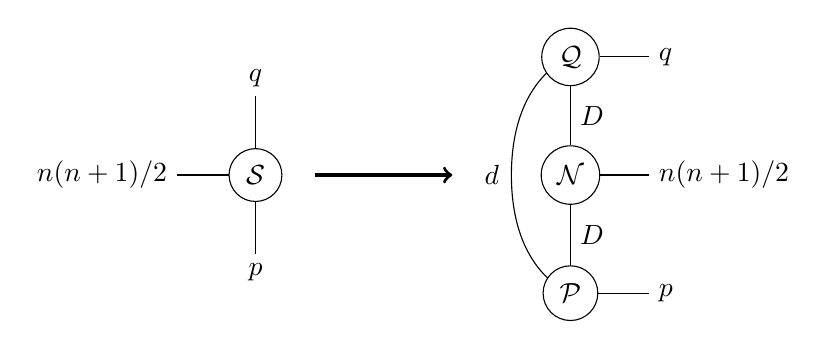
\begin{tikzpicture}
        \draw plot [smooth, tension=1.5] coordinates {(-0,-1.5) (-1.5/2,0) (-0,1.5)};
        \node[] at (-1.5/2- 0.25,0) {$d$};

        \node[draw, circle, fill=white] (S) at (-4,0) {$\tenS$};

        \node[draw, circle, fill=white] (P) at (0,-1.5) {$\tenP$};
        \node[draw, circle, fill=white] (Q) at (0,1.5) {$\tenQ$};
        \node[draw, circle, fill=white] (N) at (0,0) {$\tenN$};

        \draw[-] (P) -- (N) node[midway, right] {$D$};
        \draw[-] (N) -- (Q) node[midway, right] {$D$};

        % open legs
        \draw[-] (P) -- ++(1,0) node[right] {$p$};
        \draw[-] (Q) -- ++(1,0) node[right] {$q$};
        \draw[-] (N) -- ++(1,0) node[right] {$n(n+1)/2$};

        \draw[-] (S) -- ++(0,-1) node[below] {$p$};
        \draw[-] (S) -- ++(0,1) node[above] {$q$};
        \draw[-] (S) -- ++(-1,0) node[left] {$n(n+1)/2$};

        % draw vertical arrow from top figure (S) to bottom figure (network)
        \draw[->, very thick] (-3.25,0) -- (-1.5,0);

%
    \end{tikzpicture}
    %\begin{tikzpicture}
    %    \draw plot [smooth, tension=1.5] coordinates {(-1.5, 0) (0, 1.5/2) (1.5,0)};
    %    \node[] at (0, 1.5/2+ 0.25) {$d$};
%
    %    \node[draw, circle, fill=white] (S) at (0, 4) {$\tenS$};
%
    %    \node[draw, circle, fill=white] (P) at (-1.5, 0) {$\tenP$};
    %    \node[draw, circle, fill=white] (Q) at (1.5, 0) {$\tenQ$};
    %    \node[draw, circle, fill=white] (N) at (0, 0) {$\tenN$};
%
    %    \draw[-] (P) -- (N) node[midway, above] {$D$};
    %    \draw[-] (N) -- (Q) node[midway, above] {$D$};
%
    %    % open legs
    %    \draw[-] (P) -- ++(0, -1) node[below] {$p$};
    %    \draw[-] (Q) -- ++(0, -1) node[below] {$q$};
    %    \draw[-] (N) -- ++(0, -1) node[below] {$n(n+1)/2$};
%
    %    \draw[-] (S) -- ++(-1, 0) node[left] {$p$};
    %    \draw[-] (S) -- ++(1, 0) node[right] {$q$};
    %    \draw[-] (S) -- ++(0, -1) node[below] {$n(n+1)/2$};
%
    %    % draw vertical arrow from top figure (S) to bottom figure (network)
    %    \draw[->, very thick] (0, 2.25) -- (0, 1.5);
%
    %\end{tikzpicture}
    \caption{\label{fig:TN}Diagrammatic representation of Eq.~\eqref{eq:TN} showing the decomposition of the full tensor $\tenS$ (left) into the three tensors $\tenP$, $\tenN$, and $\tenQ$ (right). Legs are labeled with their dimension.}

\end{figure}

\begin{comment}

\section{Heat Equation}\label{sec:PDE}
We test the performance of PMMs for predicting dynamical systems described by partial differential equations.  Specifically, we consider the one-dimensional heat equation,
\begin{align}\label{eq:heat}
    \frac{\partial u(x,t)}{\partial t} = \alpha\frac{\partial^2u(x,t)}{\partial x^2}.
\end{align}
for a rod of length $L$.  For convenience, we have scaled $x$ and $t$ so that $L=1$ and the thermal diffusivity is $\alpha = 1$.  We also take the initial temperature profile to be $u(x,0)=30\sin^2(2\pi x/L)$, and the temperature at the ends of the rod to be fixed at zero, $u(0,t)=u(L,t)=0$.

The PMM we consider has the form 
\begin{equation}
\begin{aligned}
 \frac{dv_i(t)}{dt} & = -\sum_j M_{i,j} v_j(t), \\
 u_\alpha(t) & = \sum_j C_{\alpha,j}v_j(t).
\end{aligned}
\end{equation}
The initial vector $v_j(0)$ is a column vector of length $N = 5$.  The matrix $M_{i,j}$ is a $5 \times 5$ Hermitian matrix, and matrix $C_{\alpha,j}$ is a rectangular $2000 \times 5$ matrix.  The entries for $v_j(0)$, $M_{i,j}$, and $C_{\alpha,j}$ are learned by fitting the output values $u_\alpha(t)$ to the training data $u(x_\alpha,t)$.  For the training data, we take $10$ values of $t$ in the interval $[0,0.1]$ as the training data and predict $u(x_\alpha,t)$ for $t$ in the interval $(0.1,0.5]$.

We compare our PMM results with calculations using dynamic mode decomposition (DMD) method applied to the same training data utilizing the python package from Demo et al.~\cite{Demo2018}.
In Figure~\ref{fig:1D-heat} we show results of the heat equation for the one-dimensional rod.  Panel (a) shows exact temperature results for $u(x,t)$ on the left and PMM results on the right.  Panel (b) shows the relative L2 error, where the L2 norm is computed from the square-root of the sum of the squares of the individual data points.  We see that the PMM is able to describe the dynamics of the heat equation with a relative accuracy of about one part in one thousand.

Here, $\vec{v}(t) = \expm{-Mt}\vec{v}(0)$ represents the learned projected lower dimensional subspace for some $m\times m$ "Hamiltonian-like" operator $M$ , and $D$ is a $n\times m$ of "dual vectors". This formulation aims to predict $u(x_i,t)\approx d_i^\dagger(\expm{-Mt}\vec{v}(0))$.
\begin{figure*}
    \raggedright
    \begin{subfigure}{0.7\textwidth}   \includegraphics[width=\linewidth]{Figures/1dheat.pdf}
        \caption{}
        \label{fig:1D-heat_a}
    \end{subfigure}%
    \begin{subfigure}{0.4\textwidth}
        \centering
        \includegraphics[width=\linewidth]{Figures/1dheat_error.pdf}
        \caption{}
        \label{fig:1D-heat_b}
    \end{subfigure}
     \caption{Results of the heat equation for the one-dimensional rod.  Panel (a) shows exact temperature results for $u(x,t)$ on the left and PMM results on the right. Panel (b) shows the relative L2 error for both PMM and DMD, where DMD had an SVD rank $5$ truncation.}
    \label{fig:1D-heat}
\end{figure*}
%The results for applying the PMM of the form in Eq.~\eqref{eq:PMM_PDE} for a heated rod are illustrated in Figure~\ref{fig:1D-heat_a}. The heated rod has length $L=1$ discritized into 2,000 points, thermal diffusivity $\alpha = 1$, with boundary conditions  $u(0,t)=u(L,t)=0$, and initial condition $u(x,0)=30\sin(2\pi x)^2$. The training data for the PMM encompassed the first $20,000$ points for the time steps $t\in[0,0.1]$. Subsequently, The learned PMM was used to extrapolate the next $80,000$ points for the time steps $t\in[0.1,0.5]$. Remarkably, the PMM demonstrated precise learning of the evolution of the heated rod system governed by the heat equation up to its steady state as seen in Figure~\ref{fig:1D-heat_b}.

%Further research includes the exploration of real time simulation given the PMM of the form:
%\begin{align}
    %D^\dagger (\expm{-iMt}\vec{v}(0)= \vec{x}(t)
%\end{align}
%On the other hand, one can consider approximating $u(x,t)$ by the innermost eigenvalue of $M(x,t)$, like in the previous examples, where one has the PDE and the initial conditions, but no high-fidelity snapshots.
%\end{comment}
\end{comment}
\end{document}
